\chapter{Et dans le cas incompressible ? }
\renewcommand\partie{\Partie\ Chapitre \thechapter}
\label{ch-22}

\bigskip
\minitoc  

Si l'on prend la limite incompressible de la loi exacte dépendant d'une pression isotrope \eqref{eq:turb_elg_f2}, on retrouve la loi \acs{PP98} donnant le taux de cascade $\varepsilon_{PP98}$ \eqref{eq:synth_inc_EL}. Mais est-ce aussi le cas si la pression est tensorielle ? De cette question émerge une autre question : qu'est-ce qu'un système incompressible avec pression tensorielle ? Dans ce chapitre, sera présenté le travail effectué pour tenter de répondre à ces questions. Ce travail n'a pas encore été publié. 

\section{De la limite incompressible dans la loi exacte générale vers un nouveau modèle }
\label{sec-221}

Si l'on considère la limite incompressible ($\rho = \rho_0$, $\delta \rho = 0$, $\nabla \rho=0$, $\nabla \cdot \boldsymbol{v}=0$, $\nabla \cdot \boldsymbol{v_A}=0$) dans l'équation \eqref{eq:turb_cpgyr_an}, $\varepsilon_{iso}$ devient $\varepsilon_{PP98}$ et tous les termes s'annulent sauf : 
\begin{eqnarray}
\label{eq:turb_cpinc_an} 
- 4(\varepsilon - \varepsilon_{PP98}) &=& -2 \left< \delta (\overline{\boldsymbol{\Pi}}):\nabla' \boldsymbol{v'} -   \delta (\overline{\boldsymbol{\Pi}} ) :\nabla  \boldsymbol{v}\right> 
\end{eqnarray}
car la contribution de la trace de $\nabla \boldsymbol{v}$ s'annule par incompressibilité : $\overline{\boldsymbol{I}} :\nabla \boldsymbol{v} = \nabla \cdot \boldsymbol{v}=0$. On obtient ainsi une correction à la théorie PP98 dépendant de la composante anisotrope de la pression (participant à la déformation incompressible du plasma, pour plus d'information voir [\cite{cassak_pressure-strain_2022}]) : 
\begin{equation}
\label{eq:turb_cpinc_gen} \boxed{
\begin{array}{lcl}
- 4(\varepsilon - \varepsilon_{PP98}) &=& -2 \left< \delta (\overline{\boldsymbol{P}} - p \overline{\boldsymbol{I}}):\delta (\nabla \boldsymbol{v}) \right> = -2 \left< \delta \overline{\boldsymbol{\Pi}} :\delta (\nabla \boldsymbol{v}) \right>.
\end{array}}
\end{equation}
Une question émerge de ce résultat : dans des plasmas faiblement compressibles dépendant d'une pression tensorielle tels que le vent solaire, la correction anisotrope aurait-elle plus de poids que la prise en compte de la compression via les fluctuations de densité ?

Dans le cas particulier gyrotrope, on obtient :
\begin{eqnarray}
\label{eq:turb_cpinc_gyr1} 
- 4(\varepsilon - \varepsilon_{PP98}) &=& -2 \left< \delta ((p_{\parallel} - p_{\perp})(\boldsymbol{b}\boldsymbol{b} -\frac{1}{3} \overline{\boldsymbol{I}})):\delta (\nabla \boldsymbol{v}) \right> \\
\label{eq:turb_cpinc_gyr2} &=& -2 \left< \delta ((p_{\parallel} - p_{\perp})\boldsymbol{b}\boldsymbol{b}):\delta (\nabla \boldsymbol{v}) \right> .
\end{eqnarray}
On observe que la ligne \eqref{eq:turb_cpinc_gyr1} dépend de $\overline{\boldsymbol{I}} :\nabla \boldsymbol{v}$, on annule donc ce terme dans la ligne suivante \eqref{eq:turb_cpinc_gyr2}. Dans le cas incompressible, ces deux expressions sont donc équivalentes. Dans des plasmas quasi-incompressibles par contre, si l'on veut estimer le taux de cascade à l'aide de la loi exacte incompressible corrigée, les deux expressions ne seront plus équivalentes. Dans la première, on s'assure de n'utiliser que la part incompressible de la pression (la contribution de la trace de $\boldsymbol{b}\boldsymbol{b}$ étant annulée par $-\frac{1}{3} \overline{\boldsymbol{I}}$). Dans la seconde, ce n'est pas le cas, le résultat pourra alors être impacté.

On remarque que cette correction dépend de $p_{\parallel} - p_{\perp}$, c'est à dire de $\beta_{\parallel} (1-a_p)$ qui rappelle les critères d'instabilités. Dans le cas \ac{CGL}, on a vu que ces critères dépendent fortement de $\beta_{\parallel 0} (1-a_{p0})$. 
Si l'on se place dans une situation dans laquelle $\frac{\beta_{\parallel}}{2}(1 - a_p)$ serait quasiment constant, alors le terme correctif de la loi exacte à l'ordre 0 pourra s'écrire : 
\begin{eqnarray}
\label{eq:turb_cpinc_gyrlin} 
- 4(\varepsilon - \varepsilon_{PP98}) &=& -2 \left< \delta (\frac{\beta_{\parallel}}{2}(1 - a_p)\boldsymbol{v_A}\boldsymbol{v_A}):\delta (\nabla \boldsymbol{v}) \right>\\
&\simeq& - \beta_{\parallel 0}(1 - a_{p0})\left< \delta (\boldsymbol{v_A}\boldsymbol{v_A}):\delta (\nabla \boldsymbol{v}) \right> .
\end{eqnarray}
  En prenant des valeurs réalistes dans le vent solaire telles que  $\beta_{\parallel 0} \sim \num{1}$ et $|1-a_{p0}| \sim \num{0.5}$, on obtient $\varepsilon - \varepsilon_{PP98} \sim \frac{1}{8}\left< \delta (\boldsymbol{v_A}\boldsymbol{v_A}):\delta (\nabla \boldsymbol{v}) \right>  $. Si $\left< \delta (\boldsymbol{v_A}\boldsymbol{v_A}):\delta (\nabla \boldsymbol{v}) \right> \sim \varepsilon$ alors la correction de l'anisotropie de pression sera de l'ordre de $\SI{12}{\%}$ du taux de cascade $\varepsilon_{PP98}$. Près du critère firehose ($\frac{\beta_{\parallel}}{2}(1 - a_p)\sim 1$), le niveau de cette contribution sera autour de $\SI{50}{\%}$. Dans le vent solaire, d'après [\cite{hadid_energy_2017}], la contribution de la compression est de l'ordre de $\SI{10}{\%}$ de $\varepsilon_{PP98}$, c'est-à-dire plus faible que nos estimations. Le résultat très approximatif obtenu ici va dans le sens d'une correction anisotrope plus significative qu'une correction compressible, en particulier près du critère d'instabilité firehose. Si l'on regarde le diagramme publié par [\cite{osman_proton_2013}] (voir la \figref{fig:diag_osman}), suivant son signe que l'on ne peut pas estimer ici, cette contribution pourrait venir accroître ou réduire la dispersion des valeurs du taux de cascade. Bien évidemment, cette petite estimation est loin d'être suffisante pour conclure sur l'impact des anisotropies de pression sur le taux de cascade. Simulation et étude comparative dans le vent solaire sont nécessaires.

Par curiosité, on s'est demandé quelle était la physique derrière notre terme correctif. Dans le cadre des modèles incompressibles avec pression isotrope, le seul mode existant est le mode d'Alfvén qui constitue la brique fondamentale de la turbulence \ac{MHD} décrite par PP98. Notre terme correctif serait-il une trace de la correction du mode d'Alfvén pouvant induire l'instabilité firehose dans la cascade non-linéaire incompressible ? 

Afin de répondre à cette question, nous avons voulu vérifier dans un modèle incompressible dépendant d'une pression gyrotrope si le mode d'Alfvén-firehose existait. Mais aucune trace d'un modèle incompressible avec pression tensorielle n'a été trouvée dans la littérature. En fait, si l'on approche le problème sous un autre angle, celui des fermetures, on se rend compte que le cadre gyrotrope est habituellement abordé à travers la fermeture \ac{CGL}. Ajouter une fermeture incompressible signifierait alors, surcontraindre le système : une équation de trop par rapport au nombre de variables. La viabilité du système résultant en tant que modèle réaliste serait remise en cause. % Par contre, on peut y appliquer l'incompressibilité telle une limite comme on le discutera dans la section \ref{sec-224}.

\section{Proposition d'un modèle incompressible gyrotrope}
\label{sec-222}

Nous avons construit un nouveau modèle en partant de la question : comment décrire un écoulement magnétisé et incompressible dépendant d'une pression gyrotrope ? 

Dans un tel écoulement, la contrainte  $\rho = \rho_0$ et donc $\nabla \cdot \boldsymbol{v}=0$ s'impose. Elle induit pour le champ magnétique $\nabla \cdot \boldsymbol{v_A} = 0$. On a aussi besoin d'une équation sur la vitesse (premier moment) et d'une équation sur le champ magnétique (équation d'induction). L'hypothèse d'une pression gyrotrope va s'exprimer dans l'équation sur la vitesse à travers $\nabla \cdot \overline{\boldsymbol{P}}$. On a alors $\num{7}$ équations (la contrainte incompressible, les trois composantes de la vitesse et les trois composantes du champ magnétique) pour $\num{8}$ variables scalaires (les composantes de la vitesses et du champ magnétique, et les pressions parallèles et perpendiculaires). Il manque donc une équation pour fermer le système. Afin de maintenir la cohérence avec la définition de l'énergie interne telle que $u = \frac{1}{2 \rho_0} (2p_{\perp} + p_{\parallel}) $, nous avons décidé de fermer le système avec l'équation sur la trace du tenseur de pression avec $\nabla \cdot \boldsymbol{q} = 0$. Ce système est donc compatible avec la loi exacte \eqref{eq:turb_cpinc_gyr1}.

Par conséquent, le modèle incompressible gyrotrope envisagé est : 
\begin{eqnarray}
\label{eq:model_cpginc_r} \nabla \cdot \boldsymbol{v} = 0  \qquad \nabla \cdot \boldsymbol{v_A} &=& 0,\\
\label{eq:model_cpginc_v} \partial_t  \boldsymbol{v} + \nabla \cdot (\boldsymbol{v}\boldsymbol{v} - \boldsymbol{v_A}\boldsymbol{v_A} + \frac{1}{\rho_0} \overline{\boldsymbol{P_*}})  &=& 0 , \\
\label{eq:model_cpginc_p} \partial_t p + \nabla \cdot (p \boldsymbol{v} ) + \frac{2}{3} \overline{\boldsymbol{\Pi}} : \nabla \boldsymbol{v}   &=& 0  , \\
\label{eq:model_cpginc_b} \partial_t \boldsymbol{v_A} -  \nabla \cdot (\boldsymbol{v_A}\boldsymbol{v} - \boldsymbol{v}\boldsymbol{v_A}) &=& 0 ,
\end{eqnarray}
avec :
\begin{eqnarray*} 
\overline{\boldsymbol{P}} &=& p \overline{\boldsymbol{I}} +  \overline{\boldsymbol{\Pi}} =\frac{1}{3} (2 p_{\perp} + p_{\parallel} )\overline{\boldsymbol{I}} + (p_{\parallel} - p_{\perp})(\boldsymbol{b}\boldsymbol{b} - \frac{1}{3} \overline{\boldsymbol{I}} ) ,\\
 \nabla \cdot \overline{\boldsymbol{P_*}} &=& \nabla (p_{\perp}+\frac{1}{2} \rho_0\boldsymbol{v_A}^2) + \boldsymbol{b}\boldsymbol{b} \cdot \nabla (p_{\parallel}-p_{\perp}) + (p_{\parallel}-p_{\perp})\frac{1}{\boldsymbol{v_A}^2} (\boldsymbol{v_A} \cdot \nabla \boldsymbol{v_A} - 2 \boldsymbol{v_A}\boldsymbol{b}\boldsymbol{b}:\nabla \boldsymbol{v_A}),\\
 \overline{\boldsymbol{\Pi}} : \nabla \boldsymbol{v} &=& (p_{\parallel} - p_{\perp})\boldsymbol{b}\boldsymbol{b}: \nabla \boldsymbol{v}.
\end{eqnarray*}

Nous proposons de linéariser ce nouveau modèle afin d'en identifier les modes propres, et a minima vérifier que le mode d'Alfvén-firehose en est une solution. Sa forme linéaire, obtenue en suivant la méthode résumée section \ref{synt-11}, est : 
\begin{eqnarray}
\label{eq:lin_cpginc_r}0&=& k_{\perp} v_{1x} + k_{\parallel} v_{1z},\\
\label{eq:lin_cpginc_vx} 0&=&-\omega  v_{1x} ,
+  \frac{p_{\perp 1}}{\rho_0} k_{\perp}   
 + (\frac{p_{\parallel 0}-p_{\perp 0}}{\rho_0 v_{A0}^2}-1) v_{A0}k_{\parallel}v_{A1x}+  v_{A0}  k_{\perp} v_{A1z},\\
 \label{eq:lin_cpginc_vy} 0&=&-\omega  v_{1y}   + (\frac{p_{\parallel 0}-p_{\perp 0}}{\rho_0 v_{A0}^2}-1) v_{A0}k_{\parallel}v_{A1y} ,
 \\
\label{eq:lin_cpginc_vz} 0&=&-\omega  v_{1z}
+ \frac{p_{\parallel 1}}{\rho_0}k_{\parallel} 
 -  \frac{p_{\parallel 0}-p_{\perp 0}}{\rho_0 v_{A0}^2} v_{A0}  k_{\parallel} v_{A1z}, \\
\label{eq:lin_cpginc_p}0&=& -\omega  (2p_{\perp 1}+ p_{\parallel 1})   + 2 (p_{\parallel 0} - p_{\perp 0}) k_{\parallel}v_{1z}    , \\
\label{eq:lin_cpginc_b}0&=& -\omega  \boldsymbol{v_{A1}} -   k_{\parallel} v_{A0}\boldsymbol{v_1}  .
\end{eqnarray}

Après quelques manipulations, ce système peut s'écrire sous l'équation de dispersion $\overline{\boldsymbol{M}} \cdot \boldsymbol{v_1} = 0 $ avec la matrice 
\begin{equation}
 \overline{\boldsymbol{M}} =   \begin{pmatrix}
\label{eq:lin_inccpg_eqdis}  k_{\perp}  & 0 &   k_{\parallel}\\
    0 & \omega^2 - F v^2_{A0}k^2_{\parallel}  & 0 \\
    0 & 0 &  \omega^2( k^2_{\perp}  - 2 k^2_{\parallel}) - (G k^2_{\perp} + 2F k^2_{\parallel}) v^2_{A0} k^2_{\parallel}
    \end{pmatrix} .
\end{equation}
En notant $ F  =  1 - \frac{\beta_{\parallel 0}}{2} (1-a_{p0})$ et $G = 3\frac{\beta_{\parallel 0}}{2} (1-a_{p0}) -2$.

La relation de dispersion est donc : 
\begin{equation}
  \label{eq:disp_newmodel}  (\omega^2 - F v^2_{A0}k^2_{\parallel}) (\omega^2( k^2_{\perp}  - 2 k^2_{\parallel}) - (G k^2_{\perp} + 2F k^2_{\parallel}) v^2_{A0} k^2_{\parallel}) = 0 .
\end{equation}

On retrouve le mode d'Alfvén incompressible firehose $\omega_A = \pm k_{\parallel} v_{A0} \sqrt{F} $ polarisé suivant $(0,1,0)$. Cette solution s'exprime à travers les différentes quantités : 
\begin{eqnarray}
    \boldsymbol{v_{1}} &=& (0,1,0),\\
  \boldsymbol{v_{A1}} &=&  \pm  \frac{1}{\sqrt{F}} \boldsymbol{v_1} = \pm  \frac{1}{\sqrt{1 - \frac{\beta_{\parallel 0}}{2} (1-a_{p0})}} \boldsymbol{v_1} , \\
   p_{\parallel 1} &=&  (2F-1) \rho_0  v_{A0} v_{A1z} = 0,\\
   p_{\perp 1} &=& \rho_0 v_{A0} v_{A1z} = 0 .
\end{eqnarray}
On retrouve bien le comportement du mode d'Alfvén incompressible au niveau des pressions et la relation linéaire entre la vitesse et le champ magnétique. On note que cette relation est altérée par le critère firehose. On remarque que les fluctuations de pressions sont nulles (c'est aussi le cas dans le cadre \ac{CGL} [\cite{hunana_introductory_2019}]). Les seules fluctuations accompagnant ce mode sont celles de $v_{1y}$ et $v_{A1y}$. L'existence du mode Alfvén-firehose dans ce nouveau modèle incompressible donne une assise plus sérieuse à la correction trouvée de \acs{PP98}. Une surprise nous attend : un nouveau mode émerge de la relation de dispersion  \eqref{eq:disp_newmodel}. 

Ce nouveau mode, polarisé suivant $(1,0,-\tan \theta)$, est : 
\begin{equation}
    \omega_N = \pm \sqrt{ \frac{G k^2_{\perp} + 2F k^2_{\parallel}}{k^2_{\perp}  - 2 k^2_{\parallel}}} v_{A0} k_{\parallel}= \pm \sqrt{ \frac{(3\frac{\beta_{\parallel 0}}{2} (1-a_{p0}) -2) k^2_{\perp} + 2( 1 - \frac{\beta_{\parallel 0}}{2} (1-a_{p0})) k^2_{\parallel}}{k^2_{\perp}  - 2 k^2_{\parallel}}} v_{A0} k_{\parallel} 
\end{equation} 

Les différentes quantités sont alors : 
\begin{eqnarray}
\boldsymbol{v_{1}} &=& (1,0,-\tan \theta)\\
  \boldsymbol{v_{A1}} &=&  \pm  \sqrt{ \frac{k^2_{\perp}  - 2 k^2_{\parallel}}{G k^2_{\perp} + 2F k^2_{\parallel}}} \boldsymbol{v_1} \\
   p_{\parallel 1} &=& \frac{(G + F - 1) k^2_{\perp}  + 2 k^2_{\parallel} }{k^2_{\perp}  - 2 k^2_{\parallel}}   \rho_0 v_{A0}v_{A1z} = \frac{(\beta_{\parallel 0} (1-a_{p0}) -2 ) k^2_{\perp}  + 2 k^2_{\parallel} }{k^2_{\perp}  - 2 k^2_{\parallel}}   \rho_0 v_{A0}v_{A1z} \nonumber\\ && \\
   p_{\perp 1} &=& \frac{\rho_0}{k^2_{\perp} }  \frac{4F k^2_{\parallel} k^2_{\parallel} +(G  - F + 2 )k^2_{\perp} k^2_{\parallel}- k^2_{\perp} k^2_{\perp}  }{k^2_{\perp}  - 2 k^2_{\parallel}} v_{A0}v_{A1z} \nonumber\\
   &=&    \frac{(2\beta_{\parallel 0} (1-a_{p0})  -  1   )(k^2_{\perp}  -  k^2_{\parallel}) k^2_{\parallel} + 3k^2_{\parallel}k^2_{\parallel} - k^2_{\perp} k^2_{\perp}  }{k^2_{\perp} (k^2_{\perp}  - 2 k^2_{\parallel})}\rho_0 v_{A0}v_{A1z} 
\end{eqnarray}
On retrouve des résultats similaires au mode pseudo-alfvénique donnant une pression non nulle proportionnelle à $v_{A1z}$ mais avec des facteurs portant une dépendance angulaire complexes mêlées à l'anisotropie de pression moyenne.  Considérer une gyrotropie de pression lève donc la dégénérescence observée dans le cas incompressible avec pression isotrope (voir Chapitre \ref{ch-11}) similairement à la levée de dégénérescence menant aux modes magnétosonores dans le compressible. Ce nouveau mode s'accompagnant de fluctuation des pressions, qui ne sont pas identiques, il pourra engendrer des fluctuations du taux d'anisotropie de pression. Son apport au taux de cascade turbulent pourrait alors s'exprimer à travers notre terme correctif qui dépendrait des fluctuations de pression. Il pourrait aussi interagir non linéairement avec le mode d'Alfvén-firehose\footnote{Dans le futur, il serait intéressant de les étudier avec des méthodes de turbulence d'ondes par exemple.}. 

Ce modèle proposé admet donc deux modes linéaires. Ils forment donc deux canaux potentiels de développement de la cascade turbulente à l'image des modes d'Alfvén et pseudo-alfvénique dans la turbulence \ac{MHD} incompressible. Par curiosité, une étude comparative et paramétrique des modes d'Alfvén-firehose et du nouveau mode a été menée. Elle est résumée dans la section \ref{sec-223}.

\section{Etude paramétrique des modes linéaires du modèle incompressible gyrotrope } \label{sec-223}

La linéarisation du système d'équation incompressible gyrotrope proposé a abouti aux deux modes que l'on peut exprimer en fonction de $\theta$ : 
\begin{itemize}
    \item le mode d'Alfvén-firehose : $\omega =  \omega_A$ avec $\frac{\omega^2_A}{v^2_{A0}k^2_{\parallel}} = F $ et $F = 1 - \frac{\beta_{\parallel 0}}{2}(1-a_{p0})$,
    \item un nouveau mode : $\omega = \omega_N$ avec $\frac{\omega^2_N}{v^2_{A0}k^2_{\parallel}} =  \frac{G \sin^2 \theta - 2F \cos^2 \theta}{ \sin^2 \theta - 2 cos^2 \theta} $ et $G =  3\frac{\beta_{\parallel 0}}{2}(1-a_{p0}) -2$
\end{itemize}
Le mode d'Alfvén-firehose qui s'écrit $\omega_A = \pm \sqrt{F } v_{A0} k_{\parallel} $ est linéaire en $v_{A0} k_{\parallel}$ avec une pente dépendant de $a_{p0}$ et $\beta_{\parallel 0}$. Le nouveau mode est aussi  linéaire en $v_{A0} k_{\parallel}$  mais sa pente va aussi dépendre de $\theta$.  
Ils sont représentés sur la \figref{fig:lin_omega_k}  normalisé par $\omega_{ci}$ la pulsation cyclotron des ions, et en fonction de $k_{\parallel}d_i = k_{\parallel} v_{A0}/ \omega_{ci} $ avec $d_i$ la longueur inertielle ionique. Le mode d'Alfvén-firehose est représenté en bleu et le nouveau mode dans des couleurs chaudes (orange pour $\theta = \ang{25}$ et rouge pour $\theta=\ang{70}$).
\begin{figure}[!ht]
 \centering
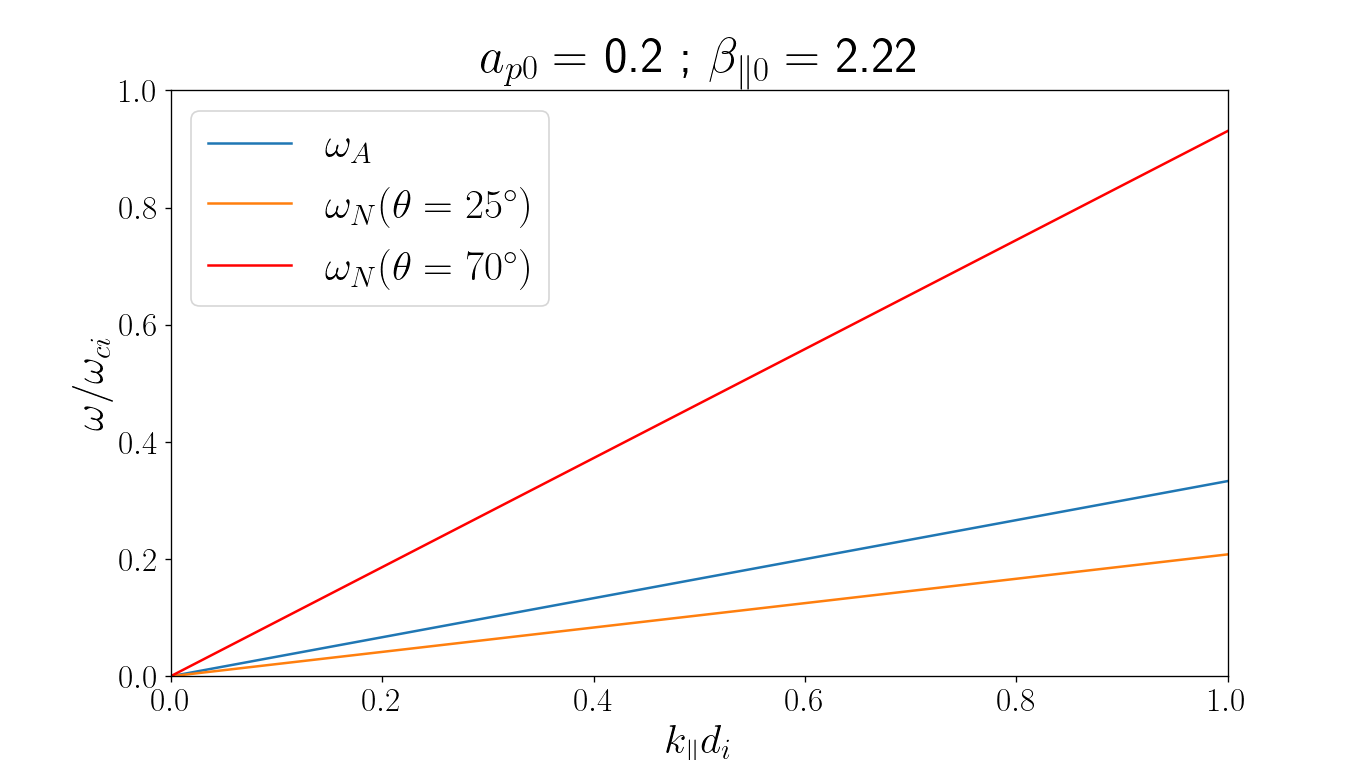
\includegraphics[width=0.8\linewidth,trim=2cm 0cm 3cm 1cm, clip=true]{./Part_2/images/lin_omega_k}
\caption{Mode d'Alfvén-firehose ($\omega_A$, bleu) et nouveau mode ($\omega_N $, orange pour $\theta = \ang{25}$ et rouge pour $\theta=\ang{70}$) normalisés par $\omega_{ci}$ la pulsation cyclotron des ions et représentés en fonction de $k_{\parallel}d_i$, avec $d_i = v_{A0}/ \omega_{ci}$, la longueur inertielle ionique. } 
\label{fig:lin_omega_k}
\end{figure}
On remarque que le nouveau mode peut être plus lent ou plus rapide que le mode d'Alfvén-firehose en fonction de $\theta$. Ce n'est pas montré ici, mais il peut aussi devenir instable quand le mode d'Alfvén-firehose est stable. Ils sont donc très différents. Ces observations, nous ont amené à faire une étude paramétrique en fonction de $\theta$ de la vitesse de phase et du taux de croissance/amortissement des instabilités. 

Au cours de cette étude, on a observé cinq comportements différents pour le nouveau mode suivant la valeur du couple  $\{\beta_{\parallel 0};a_{p0}\}$ . Ces comportements sont résumés sur la figure \ref{fig:lin_omega_theta} à travers cinq couples représentatifs. 
\begin{figure}[!ht]
 \centering
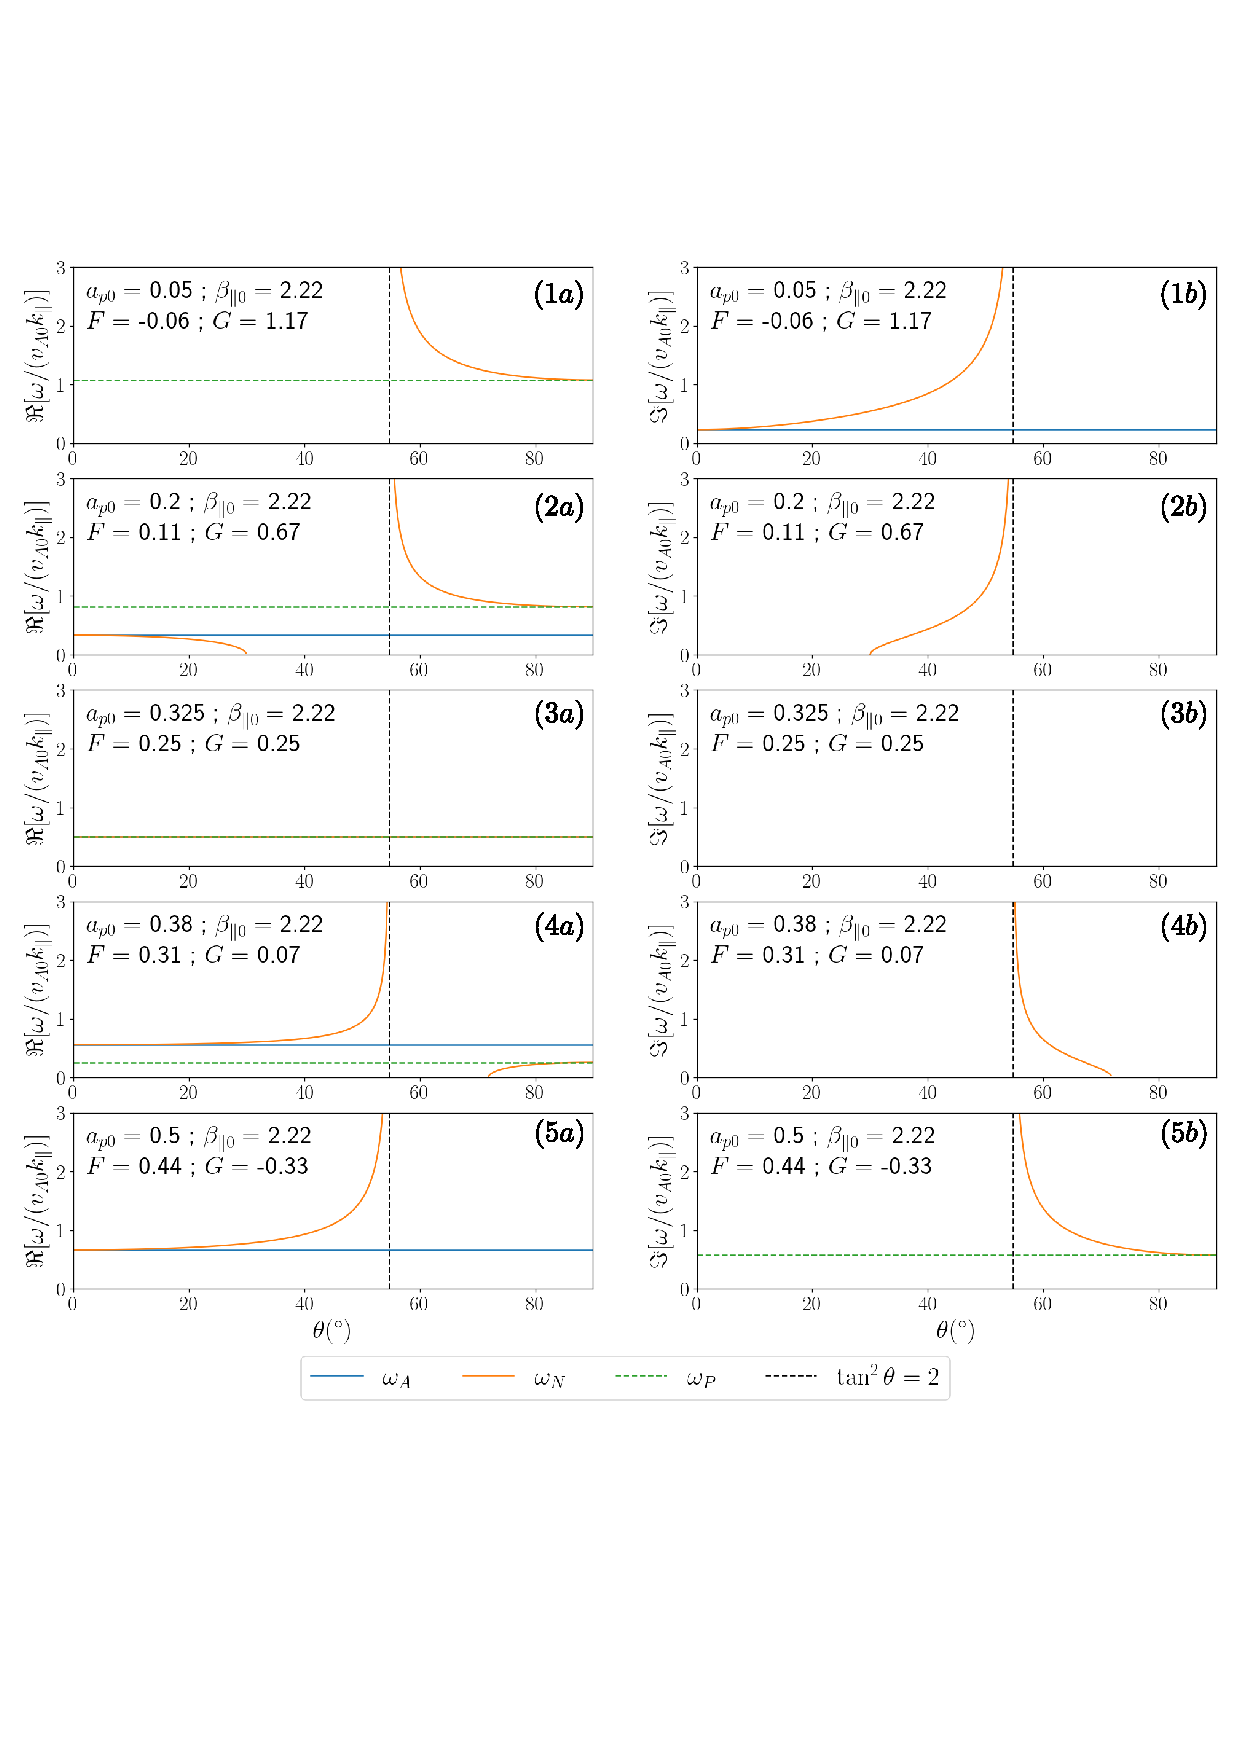
\includegraphics[width=\linewidth,trim=0.5cm 6cm 0cm 3cm, clip=true]{./Part_2/images/lin_omega_theta}
\caption{Vitesse de phase $\Re[\omega/(kv_{A0})]$ (colonne a) et taux de croissance des instabilités $\Im[\omega/(kv_{A0})]$ (colonne b) normalisées par $v_{A0}$ en fonction de l'angle $\theta$ pour le nouveau mode incompressible ($\omega_N$, orange) et pour le mode d'Alfvén ($\omega_A$, bleu). Des asymptotes sont tracées en lignes discontinues. En vert : mode asymptotique $\omega_P$. En noir : angle asymptotique $\theta_2$. Première ligne : couple (1) tel que $a_{p0} = 0.05$, $\beta_{\parallel 0} = 20/9 \Rightarrow$ instabilité firehose ($F<0$). Deuxième ligne : couple (2) tel que $a_{p0} = 0.2$, $\beta_{\parallel 0} = 20/9 $. Troisième ligne : couple (3) tel que $a_{p0} = 0.325$, $\beta_{\parallel 0} = 20/9 \Rightarrow$ seul cas stable pour tout $\theta$ ($F=G$). Quatrième ligne : couple (4) tel que $a_{p0} = 0.38$, $\beta_{\parallel 0} = 20/9  $. Cinquième ligne : couple (5) tel que $a_{p0} = 0.5$, $\beta_{\parallel 0} = 20/9  \Rightarrow$ instabilité pseudo-firehose perpendiculaire ($G<0$). Sauf graphique (3a) où tous les modes coincident, lorsque qu'un mode disparaît d'un graphique de la colonne a, il apparaît sur le graphique de la colonne b.}
\label{fig:lin_omega_theta}
\end{figure}
Sur l'ensemble de graphiques de la \figref{fig:lin_omega_theta} sont tracés en fonction de $\theta$, pour les cinq couples représentatifs et chaque mode, la partie réelle de $\omega$ normalisée par le mode d'Alfvén, $\Re[\omega/(k_{\parallel}v_{A0})]$ (colonne a) correspondant à sa vitesse de phase, ainsi que sa partie imaginaire ($\Im[\omega/(k_{\parallel}v_{A0})]$, colonne a), qui correspond au taux de croissance. $\omega$ étant ou réel ou purement imaginaire, ces graphiques sont complémentaires : si le mode est instable, il apparaîtra sur la colonne b, et s'il est stable sur la colonne a (à l'exception du graphique (3a) où les modes coîncident). Le caractère instable firehose du mode d'Alfvén (bleu) est ainsi retrouvé lorsque $F<0$ sur le graphique (1b). 

Le nouveau mode semble tendre asymptotiquement vers le mode d'Alfvén pour $\theta \sim \ang{0}$ et vers l'asymptote $\omega_P = \pm k_{\parallel}v_{A0} \sqrt{G}$ représentée par une ligne discontinue verte, pour $\theta \sim \ang{90}$. Une asymptote angulaire est aussi visible en un angle que l'on note $\theta_2$, on verra par la suite que cet angle est solution de $\tan^2 \theta = 2$. La stabilité du nouveau mode à une dépendance forte en $\theta$ : pour tout couple, il existe une gamme angulaire telle que le mode soit stable et, à l'exception du couple (3), une gamme telle que le mode est instable. 

On propose maintenant de démontrer les comportements identifiés pour le nouveau mode en fonction de $a_{p0}$ et $\beta_{\parallel 0}$. Au fil de cette analyse, on va construire le diagramme de la \figref{fig:lin_cases_update}. Les emplacements des différents couples présentés sur la \figref{fig:lin_omega_theta} sont indiqués par des croix rouges. 

\paragraph{Etude asymptotique angulaire : }Si $\theta \rightarrow \ang{0}$ ($k_{\parallel}\gg k_{\perp}$), alors $\frac{\omega^2_N}{v^2_{A0}k^2} \rightarrow F \cos^2 \theta$. La convergence vers le mode d'Alfvén-firehose du nouveau mode observée en $\theta \rightarrow \ang{0}$ sur la \figref{fig:lin_omega_theta} est ainsi vérifiée. Comme cette limite peut être stable ou instable en fonction du signe de $F$, on a représenté sur la \figref{fig:lin_cases_update}, la frontière $F=0$ en bleue et bleutée la zone où $F<0$. On retrouve dans ce comportement stable/instable l'instabilité firehose <<parallèle>> qui est présente par exemple pour le mode lent dans le cadre compressible. Le couple (1), tel que $F<0$, est un exemple instable : le nouveau mode et le mode d'Alfvén apparaîssent dans la colonne du taux de croissance (graphique (1b)). 

Si $\theta \rightarrow \ang{90}$ ($k_{\perp}\ll k_{\parallel} $), alors $\frac{\omega^2_N}{v^2_{A0}k^2} \rightarrow G \cos^2 \theta$. On retrouve l'asymptote $\omega_P$ et tracé en vert sur la \figref{fig:lin_omega_theta}. Il est instable si $G<0$. La comparaison de $G$ et $F$, qui ont la même structure à un facteur $3/2$ et un signe près, nous inspirant, on appellera cette instabilité <<instabilité pseudo-firehose perpendiculaire>>\footnote{Cette dénomination n'est proposée qu'à cause de la similarité des critères d'instabilités. Le comportement des quantités d'ordre 1 n'a pas été vérifié.}. Elle apparaît pour le couple (5) (graphique (5b)). Sur la \figref{fig:lin_cases_update}, on indique la frontière $G=0$ en vert et la zone où $G<0$ par une aire verte. 

{\bf Ainsi grâce à $F$ et $G$, on peut déduire qu'une instabilité pourra se développer dans le système pour tout couple $\{\beta_{\parallel 0};a_{p0}\}$ tel que $\frac{2}{3}>\frac{\beta_{\parallel 0}}{2}(1-a_{p0})$ (instabilité pseudo-firehose perpendiculaire, couple (5) et aire verte sur \figref{fig:lin_cases_update}) ou $\frac{\beta_{\parallel 0}}{2}(1-a_{p0})>1$ (instabilité firehose parallèle, couple (1) et aire bleue sur \figref{fig:lin_cases_update}).} Dans la zone intermédiaire (blanche sur la \figref{fig:lin_cases_update}), $G>0$ et $F>0$. 

\paragraph{Etude angulaire complète du nouveau mode : } Pour les angles $\theta$ plus obliques, le comportement de $\omega_N$ est plus difficile à établir, le signe de $\sin^2 \theta - 2 \cos^2 \theta$ venant compenser le signe de $G \sin^2 \theta - 2F \cos^2 \theta$. Une instabilité, entre l'instabilité firehose parallèle et l'instabilité pseudo-firehose perpendiculaire, pourra émerger. On la nommera <<instabilité pseudo-firehose oblique>>. Elle apparaît pour les couples (2) (graphique (2b)) et (4) (graphique (4b)). La condition d'instabilité est obtenue pour $F$ et $G$ tels que :  
\begin{eqnarray}
    (\tan^2 \theta - 2 )(G \tan^2 \theta - 2F ) &<& 0  .
\end{eqnarray}
$g(\theta) = (\tan^2 \theta - 2 )(G \tan^2 \theta - 2F )$ est une parabole présentant deux racines : 
\begin{itemize}
    \item $\tan^2 \theta = 2 $ en laquelle $\omega^2_N \rightarrow \infty$ (asymptote verticale indiquée en pointillés sur \figref{fig:lin_omega_theta}), on la note $\theta_2$,
    \item $\tan^2 \theta = 2\frac{F}{G}$ en laquelle $\omega^2_N \rightarrow 0$, on la note $\theta_{F/G}$.
\end{itemize}
La stabilité du nouveau mode dépendra donc de la position de $\theta$ par rapport à $\theta_2$ et $\theta_{F/G}$. 

Pour que le nouveau mode soit stable pour tout $\theta$, il faut $g(\theta)>0$ pour tout $\theta$. Cela n'est possible que si $F=G$, alors $g(\theta) = (\tan^2 \theta - 2 )^2 >0$. Dans ce cas, $\omega_N = \omega_A = \omega_P$. Sur la \figref{fig:lin_cases_update}, le critère $F=G$ est indiqué par la courbe noire et il est illustré par le couple (3) (graphiques (3a) et (3b)). {\bf Par conséquent, en fonction de $a_{p0}$ et $\beta_{\parallel 0}$, le nouveau mode sera stable pour tout $\theta$ si et seulement si $ \frac{\beta_{\parallel 0}}{2}(1-a_{p0}) = \frac{3}{4} $.}

$F=G$, $G=0$ et $F=0$ découpent le diagramme de la \figref{fig:lin_cases_update} en quatre zones que l'on va étudier séparément. 

Si $G<0$ (zone verte), alors $F>0$. Dans ce cas, $g(\theta) < 0$ si $\theta > \theta_2$. Cette situation est illustrée par le couple (5) (graphiques (5a) et (5b)), instable pour tout angle supérieur à $\theta_2$. On peut raccrocher à cette condition le cas $G=0$ puisque alors $F=1/3$, et la parabole sera négative si $\tan^2 \theta > 2$. Dans ces cas, on retrouve l'instabilité pseudo-firehose perpendiculaire découverte asymptotiquement si $\theta \rightarrow \ang{90}$. On peut maintenant compléter ses conditions d'existence qui deviennent : {\bf l'instabilité pseudo-firehose perpendiculaire peut se développer si $G<0$ pour tout angle $\theta > \theta_2$}.


Si $G>0$ et $F/G>1$ (zone blanche délimitée par les courbes verte et noire), $g(\theta) < 0$ si $2\frac{F}{G} > \tan^2 \theta > 2$. Cette situation est illustrée par le couple (4) (graphiques (4a) et (4b)). L'instabilité s'y développant est l'instabilité pseudo-firehose oblique. 


Si $G>0$ et $F/G<1$ (zone blanche délimitée par les courbes bleue et noire et zone bleue), $g(\theta) < 0$ si $2 > \tan^2 \theta > 2\frac{F}{G}$. {\bf Si $F<0$, l'instabilité firehose parallèle se développe pour tout angle  $\theta < \theta_2$. } Ce cas est illustré par le couple (1) (graphiques (1a) et (1b)). Si $F>0$, la situation est illustrée par le couple (2) (graphiques (2a) et (2b)). L'instabilité visible est encore une fois l'instabilité pseudo-firehose oblique. Sa condition d'apparition est donc : {\bf l'instabilité pseudo-firehose oblique peut se développer si $G>0$ et $F>0$ mais $G\neq F$, pour tout angle $\theta$ entre $\theta_2$ et $\theta_{F/G}$}. 

\begin{figure}[!ht]
 \centering
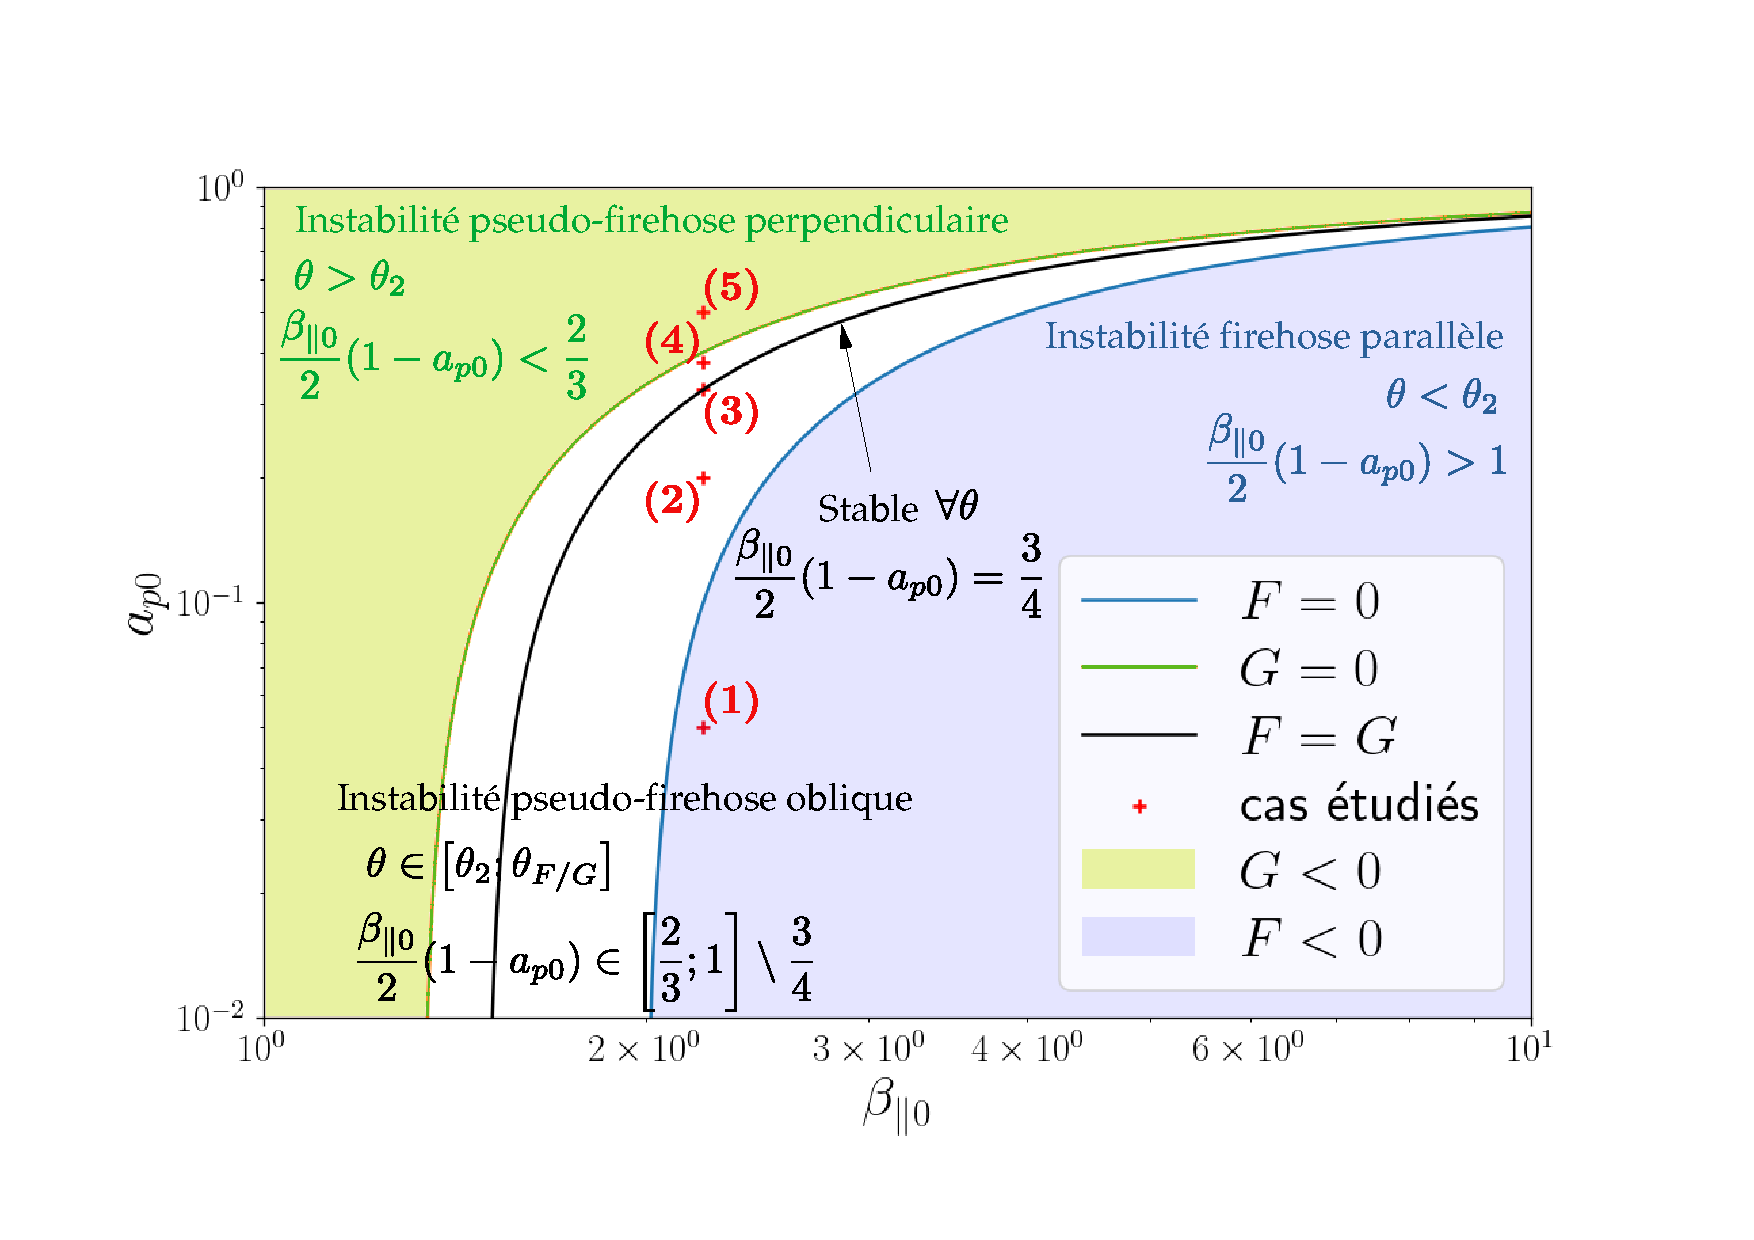
\includegraphics[width=1\linewidth,trim=2cm 1cm 3cm 2cm, clip=true]{./Part_2/images/diag_cas}
\caption{Diagramme $a_{p0}-\beta_{\parallel 0}$ résumant l'étude du nouveau mode. Croix rouges : couples $\{\beta_{\parallel 0};a_{p0}\}$ sélectionnés pour l'étude paramétrique de la \figref{fig:lin_omega_theta}. Frontière d'instabilités firehose $F=0$ (bleu) et zone instable ($F<0$, bleue) associée. Frontière d'instabilités pseudo-firehose perpendiculaire $G=0$ (verte) et zone instable ($G<0$, verte) associée. Ligne noire : ensemble des couples $\{\beta_{\parallel 0};a_{p0}\}$ stables pour tout angle $\theta$ paramétrisé par  $F=G$. Zone blanche : instabilité pseudo-firehose oblique. }
\label{fig:lin_cases_update}
\end{figure}


La zone de stabilité de ce nouveau mode en fonction des paramètres $\beta_{\parallel 0}$ et $a_{p0}$ est donc quasi-inexistante. Un résumé de l'ensemble des éléments de cette analyse est donnée sur la \figref{fig:lin_cases_update}. Sachant que la problématique principale de ce travail se place dans le cadre compressible, l'exploitation de ce modèle incompressible n'a pas été engagée mais il fera l'objet d'un nouveau papier en préparation [\cite{simon_article_2023}]. 


% \section{Limite incompressible du modèle \ac{CGL}}\label{sec-224}

% Dans le cas \ac{MHD} compressible avec pression isotrope, le mode pseudo-alfvénique apparaît comme une limite incompressible des modes compressibles magnétosonores. Similairement, on s'est demandé si l'on pouvait retrouver une trace du nouveau mode dans la limite incompressible du modèle \ac{CGL} linéaire. 

% Dans le cas linéaire, le modèle \ac{CGL} donne l'équation de dispersion \eqref{eq:lin_cpg_eqdis} que l'on va simplement noter $\overline{\boldsymbol{M}} \boldsymbol{v}_1 = 0$. Avec la contrainte incompressible $\nabla \cdot \boldsymbol{v}_1 = 0$, on peut écrire $\boldsymbol{v}_1$ sous la forme d'un potentiel vecteur $\boldsymbol{\Omega}$ : $\boldsymbol{v}_1 = \nabla \times \boldsymbol{\Omega} = \overline{\boldsymbol{N}}\boldsymbol{\Omega}$ avec $\overline{\boldsymbol{N}} = i \boldsymbol{k} \times \overline{\boldsymbol{I}} = i \begin{pmatrix} 0&-k_{\parallel}&0\\k_{\parallel}&0&-k_{\perp}\\ 0&k_{\perp}&0 \end{pmatrix} $. Le modèle \ac{CGL} linéaire surcontraint via l'incompressibilité s'exprime alors à travers l'équation de dispersion : $\overline{\boldsymbol{M}}  \overline{\boldsymbol{N}} \boldsymbol{\Omega}=0$ avec 
% \begin{equation}
%     \overline{\boldsymbol{M}} \overline{\boldsymbol{N}} = \begin{pmatrix}
% \label{eq:lin_cpginc_eqdis}  0&  -k_{\parallel}(\frac{\omega^2-\omega^2_A}{v^2_{A0}k^2_{\parallel}} -  (\frac{\beta_{\parallel 0}}{2} a_{p0} +1 ) \frac{k^2_{\perp}}{k^2_{\parallel}})  & 0  \\
%     k_{\parallel} \frac{\omega^2 - \omega^2_A}{v^2_{A0}k^2_{\parallel}}  & 0 & - k_{\perp}\frac{\omega^2-\omega^2_A}{v^2_{A0}k^2_{\parallel}}\\
%       0  &k_{\perp}(\frac{\omega^2 }{ v^2_{A0}k^2_{\parallel}} -   \frac{\beta_{\parallel 0}}{2}  (3-a_{p0})) &0 
%     \end{pmatrix} ,
% \end{equation}
% où $\omega^2_A = - v^2_{A0}k^2_{\parallel} ( \frac{\beta_{\parallel 0}}{2} (1-a_{p0})-1)$ correspond au mode d'Alfvén-firehose incompressible. On remarque que ce mode est solution si $\Omega_y = 0$, c'est-à-dire pour une polarisation de la vitesse orientée suivant $(0,1,0)$. 

% On a vu dans la section \ref{sec-222} que le nouveau mode est polarisé suivant $(\cos \theta,0,-\sin \theta)$.  Si l'on impose cette polarisation dans $\Omega$ on obtient $\Omega_y \neq 0$. Dans ce cas l'équation de dispersion peut alors s'écrire sous la forme du système :
% \begin{eqnarray}
%     \label{eq:lin_cglinc_1} k_{\parallel}(\omega^2-\omega^2_A - v^2_{A0}  (\frac{\beta_{\parallel 0}}{2} a_{p0} +1 ) k^2_{\perp}) &=& 0 ,\\
%      \label{eq:lin_cglinc_2} k_{\perp}(\omega^2  - v^2_{A0}   \frac{\beta_{\parallel 0}}{2}  (3-a_{p0}) k^2_{\parallel})&=& 0 ,\\
%      \label{eq:lin_cglinc_3} k_{\parallel}\Omega_x - k_{\perp}\Omega_z&=&0 .
% \end{eqnarray}
% On va étudier ce système en fonction de l'angle $\theta$ de propagation : 
% \begin{itemize}
%     \item $\theta = \ang{0} \Rightarrow k_{\perp} = 0$ et on suppose  $ k_{\parallel} \neq 0$, alors $\omega^2 =\omega^2_A$ et $\Omega_x =0$. On retrouve le mode firehose parallèle associé à un champ de vitesse sera polarisé suivant $(1,0,0)$.
%     \item $\theta = \ang{90} \Rightarrow k_{\parallel}  = 0$ et on suppose  $k_{\perp} \neq 0$, alors $\omega^2 =0$ et $\Omega_z =0$. On obtient un mode qui ne se propage pas et un champ de vitesse polarisé suivant $(0,0,1)$.
%     \item Si $ k_{\parallel} \neq 0$ et $k_{\perp} \neq 0$, alors $\omega^2  = v^2_{A0}   \frac{\beta_{\parallel 0}}{2}  (3-a_{p0})k^2_{\parallel}$ et $\theta$ doit vérifier $\tan^2 \theta  =\frac{2(\beta_{\parallel 0}(2-a_{p0})-1)}{\beta_{\parallel 0} a_{p0}+2}$.
% \end{itemize}
% Après quelques manipulations de $\omega^2  = v^2_{A0}   \frac{\beta_{\parallel 0}}{2}  (3-a_{p0})k^2_{\parallel}$ et de la condition $\tan^2 \theta  =\frac{2(\beta_{\parallel 0}(2-a_{p0})-1)}{\beta_{\parallel 0} a_{p0}+2}$, il est possible de faire ressortir la relation de dispersion du nouveau mode. 

% On remarque qu'appliquer la contrainte incompressible sur le modèle \ac{CGL} revient à chercher la limite telle que $p_{\parallel}$ ou $p_{\perp}$ respecte leur équation individuelle dans le modèle incompressible gyrotrope. En fait, la limite incompressible du modèle \ac{CGL} correspond à l'intersection des solutions des modèles incompressible gyrotrope défini avec la trace de la pression, incompressible gyrotrope défini avec l'équation sur $p_{\parallel}$ et incompressible gyrotrope défini avec l'équation sur $p_{\perp}$. Dans chacun de ces modèles, le mode d'Alfvén-firehose sera accompagné d'un nouveau mode dont l'expression dépend du choix de la fermeture sur la pression. Mais tous seront polarisé tel que $(\cos \theta,0,-\sin \theta)$ et peuvent être retrouvés dans le mode surcontraint du modèle \ac{CGL}. 

\newpage
\section{Synthèse : Limite incompressible et pistes d'étude}
\label{synt-22}

\fcolorbox{red}{white}{\begin{minipage}[c]{\linewidth}
\paragraph{Limite incompressible de la loi exacte avec pression tensorielle et cas gyrotrope :}
\begin{eqnarray}
    \label{eq:synth_turbinc_pgen} - 4(\varepsilon - \varepsilon_{PP98}) &=& -2 \left< \delta (\overline{\boldsymbol{P}} - p \overline{\boldsymbol{I}}):\delta (\nabla \boldsymbol{v}) \right> = -2 \left< \delta \overline{\boldsymbol{\Pi}} :\delta (\nabla \boldsymbol{v}) \right>,\\
\label{eq:synth_turbinc_pgyr} - 4(\varepsilon - \varepsilon_{PP98}) &=& -2 \left< \delta ((p_{\parallel} - p_{\perp})(\boldsymbol{b}\boldsymbol{b} -\frac{1}{3} \overline{\boldsymbol{I}})):\delta (\nabla \boldsymbol{v}) \right>.
\end{eqnarray}
$\Rightarrow$ Questionne l'existence d'un modèle incompressible gyrotrope. 


\paragraph{Modèle incompressible avec pression gyrotrope proposé compatible avec la loi exacte : }
\begin{eqnarray}
\label{eq:synth_incg_v} \partial_t  \boldsymbol{v} + \nabla \cdot (\boldsymbol{v}\boldsymbol{v} - \boldsymbol{v_A}\boldsymbol{v_A} + \frac{1}{\rho_0} \overline{\boldsymbol{P_*}})  &=& 0  ,\\
\label{eq:synth_incg_p} \partial_t p + \nabla \cdot (p \boldsymbol{v} ) + \frac{2}{3} \overline{\boldsymbol{\Pi}} : \nabla \boldsymbol{v}   &=& 0 ,  \\
\label{eq:synth_incg_b} \partial_t \boldsymbol{v_A} -  \nabla \cdot (\boldsymbol{v_A}\boldsymbol{v} - \boldsymbol{v}\boldsymbol{v_A}) &=& 0 ,\\
 \text{avec } \quad \overline{\boldsymbol{P_*}} = (p+p_m) \overline{\boldsymbol{I}} + \overline{\boldsymbol{\Pi}}, \quad p_m = \frac{\rho_0 | \boldsymbol{v_A}|^2}{2}, \quad p = \frac{1}{3} (2 p_{\perp} + p_{\parallel} ), &&  \nonumber\\ \overline{\boldsymbol{\Pi}} = (p_{\parallel} - p_{\perp})(\boldsymbol{b}\boldsymbol{b} - \frac{1}{3} \overline{\boldsymbol{I}}),  \quad \boldsymbol{b} = \frac{\boldsymbol{v_A}}{|\boldsymbol{v_A}|}, \quad \text{et} \quad \nabla \cdot \boldsymbol{v} &=&  0.  \nonumber
\end{eqnarray}

\paragraph{Etude linéaire du modèle proposé : }
\begin{itemize}
    \item Mode d'Alfvén incompressible polarisé suivant $(0,1,0)$ :
\begin{eqnarray}
\label{eq:synth_lininc_disp1}    
  \frac{\omega^2}{v^2_{A0}k^2_{\parallel}} + \frac{\beta_{\parallel 0}}{2}(1-a_{p0})-1  &=&0,\\
\text{Instabilité firehose : } \frac{\beta_{\parallel 0}}{2}(1-a_{p0})-1 &>&0 .
\end{eqnarray} 
    \item Nouveau mode polarisé suivant $(1,0,- \tan \theta)$ : (voir la \figref{fig:lin_cases_update})
\begin{eqnarray}
\label{eq:synth_lininc_disp2}    
  \frac{\omega^2}{v^2_{A0}k^2_{\parallel}} - \frac{2(\frac{\beta_{\parallel 0}}{2}(1-a_{p0})-1)\cos^2 \theta 
  +  ( 3\frac{\beta_{\parallel 0}}{2}(1-a_{p0}) - 2) \sin^2 \theta}{\sin^2 \theta-2\cos^2 \theta}  =0. && \\
\text{Critère d'instabilité pseudo-firehose : }  \frac{\beta_{\parallel 0}}{2}(1-a_{p0}) \neq \frac{3}{4}. && 
\end{eqnarray} 
\end{itemize}

% \paragraph{\\Limite incompressible du modèle \ac{CGL} :}
% \begin{itemize}
%     \item Survie du mode d'Alfvén-firehose $\Rightarrow$ Solution non-linéaire, pendant gyrotrope du mode d'Alfvén non linéaire ?
%     \item Apparition d'un mode surcontraint correspondant au nouveau mode incompressible.
% \end{itemize}

Les résultats obtenus ici à propos du nouveau modèle semble prometteur et feront l'objet d'une publication future. 
\end{minipage}}
